\apendice{Plan de Proyecto Software}

\section{Introducción}

\section{Planificación temporal}
La planificación temporal del proyecto se ha seguido con la realización de los \textit{sprints} marcados en cada reunión.

\subsubsection{\textit{Sprint} 1: \textit{Sprint} inicial}
Fechas: 28 febrero 2023 -- 7 marzo 2023.
\begin{itemize}
\item\textbf{Planificación del \textit{sprint}}

En la reunión de planificación del sprint se fijaron las siguientes tareas:
\begin{enumerate}
	\item Configuración inicial del repositorio
	\item Prototipos de las vistas de la aplicación
	\item Creación diagrama entidad-relación
\end{enumerate}

\item\textbf{\textit{Burndown Report}}

\begin{figure}
	\centering
	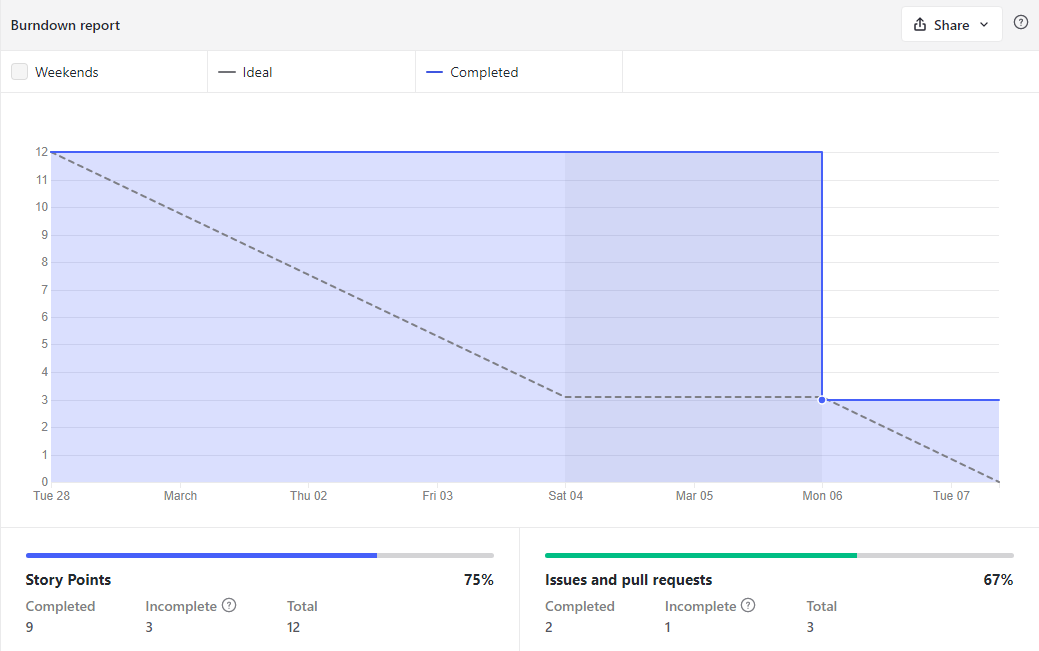
\includegraphics[width=\textwidth]{../img/Anexos/Sprints/Sprint1.png}
	\caption{\textit{Burndown Report Sprint 1}}\label{ReportSprint1}
\end{figure}

Como se puede apreciar en la figura~\ref{ReportSprint1}, no todas las tareas aparecen como completadas. Esto es debido a que el diagrama entidad-relación se dejó abierto ya que faltaba información para completarlo.

\item\textbf{Revisión del \textit{sprint}}

Durante la revisión se mostró el trabajo realizado y se vieron los cambios que se debían realizar en el diagrama entidad-relación que a su vez implicaban cambios en los prototipos de las vistas de la aplicación.
Se llegó a la conclusión de que podía ser buena idea dividir el diagrama E/R haciendo vistas del mismo para que fuere más fácil resolverlo.
\end{itemize}


\subsubsection{\textit{Sprint} 2: Casos de uso y diagrama E/R de cada caso}
Fechas: 7 marzo 2023 -- 14 marzo 2023.
\begin{itemize}
\item\textbf{Planificación del \textit{sprint}}

En la reunión de planificación del sprint se fijaron las siguientes tareas:
\begin{enumerate}
	\item Creación de casos de uso junto a su vista del diagrama E/R.
	\item Aprendizaje de Flask.
\end{enumerate}

\item\textbf{\textit{Burndown Report}}

\begin{figure}
	\centering
	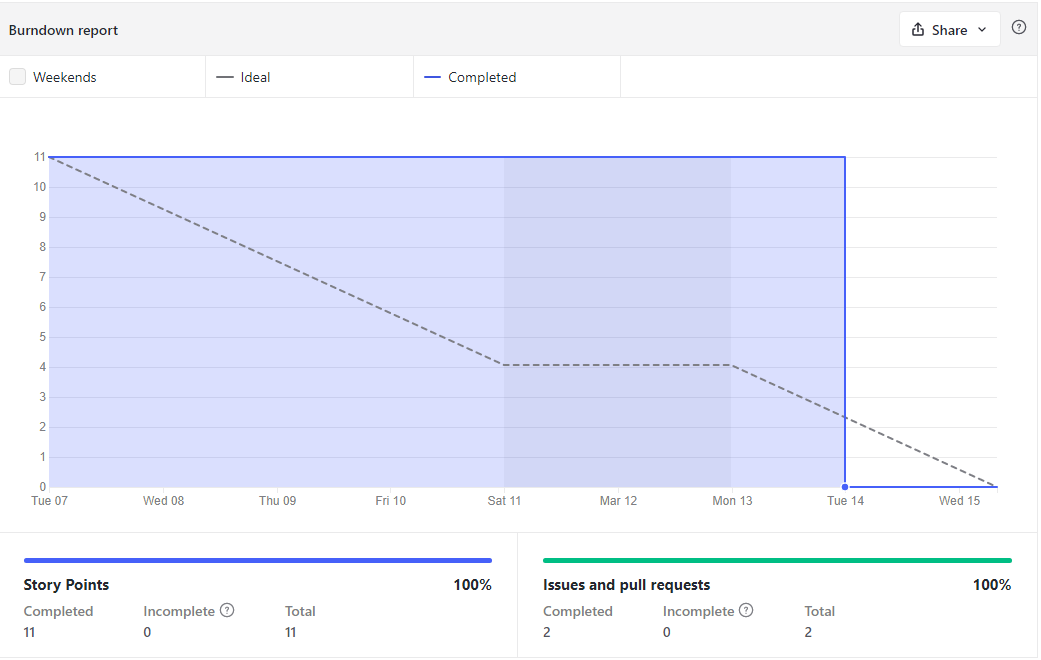
\includegraphics[width=\textwidth]{../img/Anexos/Sprints/Sprint2.png}
	\caption{\textit{Burndown Report Sprint 2}}\label{ReportSprint2}
\end{figure}

En este \textit{sprint} se completaron las tareas marcadas en el tiempo fijado durante la reunión de planificación, pero muchas cosas quedaron pendientes de cambios en futuros \textit{sprints}. En la figura~\ref{ReportSprint2} se puede ver el \textit{Burndown Report} del \textit{sprint}.

\item\textbf{Revisión del \textit{sprint}}

En la reunión de revisión se estudió de nuevo el diagrama E/R y se indicaron nuevos cambios menores en el mismo. También se propuso el comenzar a realizar el diagrama de casos de uso y continuar con el estudio de Flask.
\end{itemize}

\subsubsection{\textit{Sprint} 3: Documentación de casos de uso e investigación y aprendizaje de Flask y bibliotecas JavaScript}
Fechas: 14 marzo 2023 -- 21 marzo 2023.
\begin{itemize}
\item\textbf{Planificación del \textit{sprint}}

En la reunión de planificación del sprint se fijaron las siguientes tareas:
\begin{enumerate}
		\item Realizar el diagrama de casos de uso
		\item Cambios en las vistas adaptándolas a los casos de uso
		\item Documentar los casos de uso con sus tablas
		\item Investigar bibliotecas de JavaScript que pudiesen ayudar
		\item Aprender sobre Flask
\end{enumerate}

\item\textbf{\textit{Burndown Report}}

\begin{figure}
	\centering
	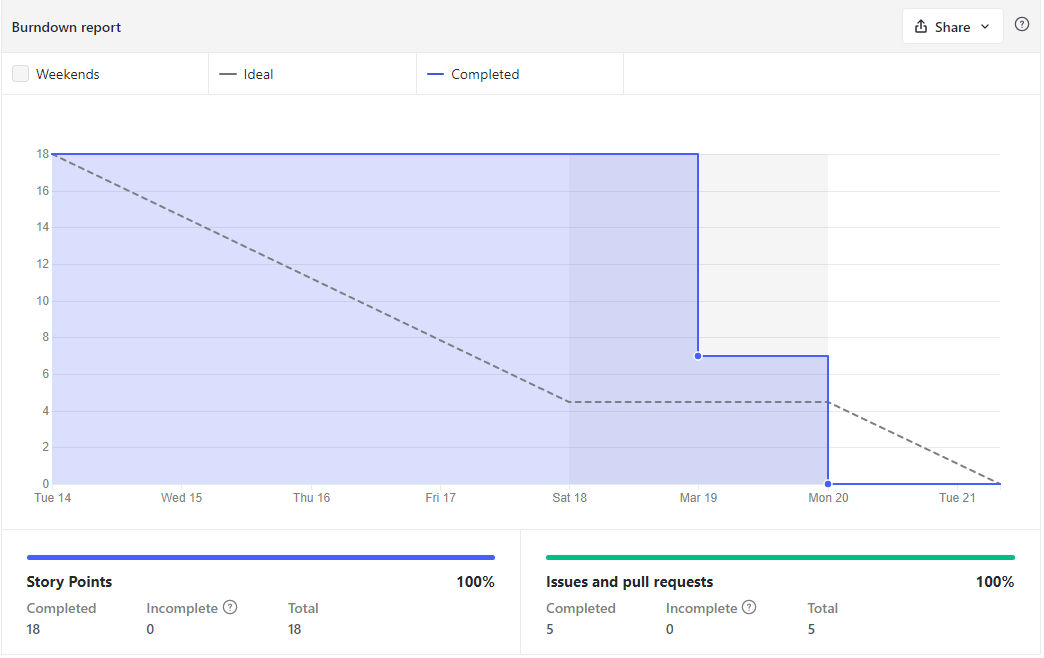
\includegraphics[width=\textwidth]{../img/Anexos/Sprints/Sprint3.png}
	\caption{\textit{Burndown Report Sprint 3}}\label{ReportSprint3}
\end{figure}

En este \textit{sprint} se completaron las tareas marcadas aunque el tiempo marcado para el aprendizaje de Flask fue menor debido a falta de tiempo durante esta semana. Estaba previsto dedicar en total 18 horas al \textit{sprint}, pero finalmente fueron 15. En la figura~\ref{ReportSprint3} se puede ver el \textit{Burndown Report} del \textit{sprint}.

\item\textbf{Revisión del \textit{sprint}}

Durante la revisión se vio que había casos de uso que no eran necesarios y que se podían añadir como excepciones de otros. Esto produjo que el diagrama de casos de uso se debía cambiar, lo que implica un cambio en la documentación de las tablas y en los prototipos de las vistas de la aplicación.
\end{itemize}

\subsubsection{\textit{Sprint} 4: Cambios en los casos de uso y vistas, documentación y Flask}
Fechas: 21 marzo 2023 -- 28 marzo 2023.
\begin{itemize}
\item\textbf{Planificación del \textit{sprint}}

En la reunión de planificación del sprint se fijaron las siguientes tareas:
\begin{enumerate}
		\item Cambios en el diagrama de casos de uso dividiendo en diagrama por niveles y crear vistas del diagrama E/R para los casos de uso.
		\item Cambios en algunos prototipos de las vistas de la aplicación.
		\item Cambios en la documentación de los casos de uso (tablas).
		\item Añadir documentación.
		\item Comenzar estructura básica de la aplicación en Flask.
\end{enumerate}

\item\textbf{\textit{Burndown Report}}

\begin{figure}
	\centering
	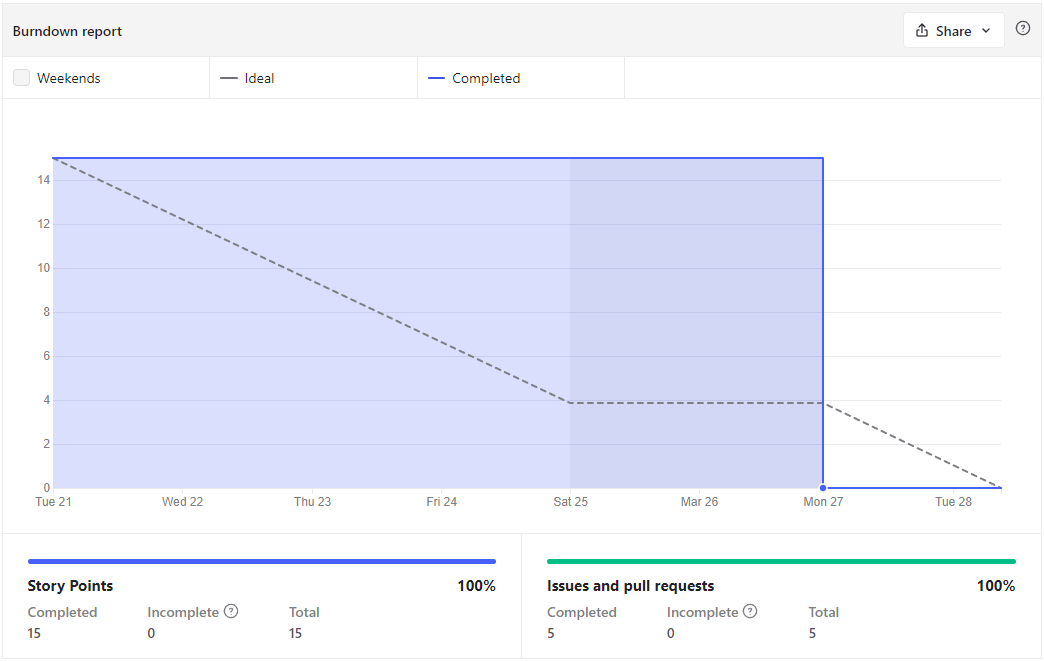
\includegraphics[width=\textwidth]{../img/Anexos/Sprints/Sprint4.png}
	\caption{\textit{Burndown Report Sprint 4}}\label{ReportSprint4}
\end{figure}

A lo largo del \textit{sprint} se realizaron la mayoría de tareas marcadas, pero en las tareas de añadir documentación y comenzar con Flask, no se hizo tanto como estaba esperado debido a la falta de tiempo. 
Se planeo que se iban a poder dedicar más horas de las que al final se dedicaron y no se avanzó todo lo planeado en estas tareas. 
Aún así, se decidió cerrarlas, ya que algo si se había avanzado, y crear de nuevo tareas similares en próximos \textit{sprints}.

La tarea de <<Cambios en el diagrama de casos de uso dividiendo en diagrama por niveles y crear vistas del diagrama E/R para los casos de uso>> tenía una previsión de 2 horas que se realizó en el plazo estimado, la tarea <<Cambios en algunos prototipos de las vistas de la aplicación>> tenía una estimación de 3 horas aunque finalmente fueron 4, la tarea <<Cambios en la documentación de los casos de uso (tablas)>> tenía marcada 4 horas de duración que finalmente fueron 5, la tarea de <<Añadir documentación>> tenía pensada una dedicación de 3 horas que al final se quedó en 1 hora y media aproximadamente y, por último, la tarea <<Comenzar estructura básica de la aplicación en Flask.>> tenía una previsión de 3 horas que quedó reducida a una media hora por falta de tiempo durante el \textit{sprint}. 
En la figura~\ref{ReportSprint4} se puede ver el \textit{Burndown Report} del \textit{sprint}.

\item\textbf{Revisión del \textit{sprint}}

En la reunión de revisión del \textit{sprint} se decidió hacer algunos cambios en los casos de uso, lo que implica un cambio en la documentación de las tablas y los prototipos de las vistas ya que el funcionamiento esperado de la aplicación cambia. También se decidió realizar algún cambio en el diagrama E/R añadiendo nuevos atributos y sacando un atributo a una nueva entidad.
\end{itemize}

\subsubsection{\textit{Sprint} 5: Documentación y comienzo de la aplicación}
Fechas: 28 marzo 2023 -- 11 abril 2023.
\begin{itemize}
\item\textbf{Planificación del \textit{sprint}}

En la reunión de planificación del sprint se fijaron las siguientes tareas:
\begin{enumerate}
		\item Cambios en el diagrama E/R y en algún caso de uso.
		\item Cambios en algunas tablas de los CU y en sus respectivas vistas.
		\item Evaluar plugins/frameworsk para tablas.
		\item Añadir documentación.
		\item Desarrollo de la aplicación.
\end{enumerate}

\item\textbf{\textit{Burndown Report}}

En este \textit{sprint} surgió un problema con herramienta ZenHub que utilizaba para llevar un seguimiento de los \textit{sprints} desde GitHub. Es una herramienta de pago que en teoría cuenta con versiones gratuitas para proyectos \textit{open source} y para profesores. Contacté con ellos para poder obtener una licencia gratuita de la herramienta, pero no fue posible conseguirla. Por lo tanto, a partir de este \textit{sprint} no pude utilizar la herramienta y no pude sacar la imagen del \textit{Burndown Report}.

Para la tarea de <<Cambios en el diagrama E/R y en algún caso de uso>> se estimaba un tiempo de realización de 1 hora que se cumplió.

Para la tarea <<Cambios en algunas tablas de los CU y en sus respectivas vistas>> se puso una estimación de 5 horas que finalmente fueron 7 horas.

Para la tarea <<Evaluar plugins/frameworsk para tablas>> se había marcado una planificación de 2 horas que se cumplió, excediendo un poco de la planificación, ya que aparte de buscar y valorar distintas librerías de JavaScript para la visualización de tablas estuve haciendo pruebas con la librería Grid.js que decidí utilizar para el proyecto.

La tarea de <<Añadir documentación>> tenía marcada una planificación de 3 horas que se cumplió dentro del plazo.

Por último, la tarea de <<Desarrollo de la aplicación>>, donde se buscaba empezar con la aplicación web, tenía una estimación de 8 horas que se convirtió en unas 10 horas de trabajo real debido a algunos problemas surgidos durante el desarrollo.

\item\textbf{Revisión del \textit{sprint}}

En la reunión de revisión se estuvo viendo el trabajo realizado durante el \textit{sprint}. En la parte de documentación se decidió que se debían hacer algunos pequeños cambios en las tablas de los casos de uso, la visualización de imágenes, cambios de orden en un diagrama y cambios en algún título.

En la parte de desarrollo de la aplicación web se decidió realizar algunos cambios en la visualización de tablas para que no ocupasen tanta pantalla así como en el menú de la web para hacerlo más pequeño introduciendo submenús. También se dijo que era mejor poner un selector de centro en la pantalla de la asignación de horas para que de esta forma ya saliesen los datos de la tabla filtrados por centro. 
\end{itemize}

\subsubsection{\textit{Sprint} 6: Base de datos y comenzar a dar funcionalidad a la web}
Fechas: 11 abril 2023 -- 24 abril 2023.
\begin{itemize}
\item\textbf{Planificación del \textit{sprint}}

En la reunión de planificación del sprint se fijaron las siguientes tareas:
\begin{enumerate}
		\item Creación de los modelos y la base de datos en base a los modelos.
		\item Crear la primera carga de la base de datos con CSV y script SQL.
		\item Creación de más vistas junto a su funcionalidad.
		\item Cambios en la documentación.
		\item Añadir más documentación.
\end{enumerate}

\item\textbf{\textit{Burndown Report}}
Este \textit{sprint} tenía una duración inicial de una semana, pero debido a falta de tiempo por exámenes y entregas de trabajos, decidí aplazar una semana más la reunión de revisión para poder trabajar en el proyecto. 
Además, se tuvo que cambiar la fecha habitual de las reuniones debido a que empecé prácticas en una empresa y ya no era compatible la hora/día que se tenía.

La primera tarea completada fue la de <<Creación de los modelos y la base de datos en base a los modelos>>. 
Se puso una estimación de 4 horas, que de trabajo real fue el doble, unas 8 horas. 
Este exceso de tiempo fue debido en gran medida a errores surgidos a la hora de crear la base de datos utilizando el \textit{ORM} SQLAlchemy. 
Los problemas eran principalmente por como hacía la carga de la base de datos que hacía que en algunos contextos estuviese disponible y en otros no, provocando errores al ejecutar la aplicación y generar las tablas de la base de datos.

La tarea <<Crear la primera carga de la base de datos con CSV y script SQL>> tenía una planificación de 2 horas....


\item\textbf{Revisión del \textit{sprint}}

\end{itemize}



\section{Estudio de viabilidad}

\subsection{Viabilidad económica}

\subsection{Viabilidad legal}


